\graphicspath{{Images/heterogeneous/}}

\chapter{Heterogeneous hydrogel structures as Miniature Hyper-redundant Soft Manipulators}
\label{chap:heterogeneous}
Stimuli-responsive hydrogels can sense environmental cues and change their volume accordingly without the need for additional sensors or actuators. This enables a significant reduction in the size and complexity of resulting devices. However, since the responsive volume change of hydrogels is typically uniform, their robotic applications requiring localized and time-varying deformations have been challenging to realize. Here, using addressable and tunable hydrogel building blocks – referred to as Soft Voxel Actuators (SVAs) –heterogeneous hydrogel structures with programmable spatiotemporal deformations is presented. SVAs are produced using a mixed-solvent photopolymerization method, utilizing a fast reaction speed and the cononsolvency property of PNIPAAm to produce highly interconnected hydrogel pore structures, resulting in tunable swelling ratio, swelling rate, and Young’s Modulus in a simple, one-step casting process that is compatible with mass production of SVA units. By designing the location and swelling properties of each voxel and by activating embedded Joule heaters in the voxels, spatiotemporal deformations are achieved which enables heterogeneous hydrogel structures to manipulate objects, avoid obstacles, generate traveling waves and morph to different shapes. Together, these innovations pave the way towards tunable, untethered, and high degree-of-freedom hydrogel robots that can adapt and respond to changing conditions in unstructured environments.
\section{Bsckground}
Smart hydrogels have attracted great interest in many different fields, such as drug delivery \citesuperscript{Annabi2014,Stuart2010},               
microfluidics \citesuperscript{DEramo2018a,Goy2019}, and soft robotics \citesuperscript{Banerjee2018}, owing to their large and reversible volume changes in response to a broad range of stimuli without using any additional sensors and actuators. This feature helps reduce the size of devices made of smart hydrogels. 
% \note{stimuli responsive are responsive to stimuli}. 
Practical soft robotic applications, ranging from basic bending and shortening primitives to complex reconfigurations, all require time-varying and local deformations of bulk hydrogels in order to approach the dexterity of 
% better mimic  the functions of 
soft organisms in performing tasks such as grasping and manipulation \citesuperscript{Ionov2014, Erol2019}.
However, the responsive volume change of smart hydrogels is typically uniform.
% \dma{\sout{to achieve precise and complex reconfigurations}}
Two main approaches have been adopted by researchers to achieve nonuniform spatiotemporal deformation in hydrogels \citesuperscript{Ionov2014}. In the first approach, heterogeneous structures in the shape of sheets and rods are fabricated by patterning material domains using manufacturing techniques such as micro- and meso-patterning \citesuperscript{Zhou2018b,Klein2007,Kim2012,Ma2016a,Erb2013,Huang2017} and 3D printing \citesuperscript{Zheng2018}. Differing swelling properties of neighboring domains upon stimulation results in nonuniform strain fields in these structures, causing them to transform into a variety of complex shapes like coils and conical helices \citesuperscript{Wu2013,Liu2016}.
% Zhou2018b,Peng2018,Lee2014,Ma2016a,Erb2013,Huang2017 of different swelling properties. Nonuniform strains develop across the \dma{\sout{bulk}} material as a result of the difference in amount of swelling of these domains. 
% Fabrication techniques used for patterning material domains include micro- and meso-patterning\citesuperscript{Zhou2018b,Peng2018,Lee2014,Ma2016a,Erb2013,Huang2017} and 3D printing.
% %may be used to create these patterns,
% \citesuperscriptsuperscript{Zheng2018} Basic shapes such as sheets and rods, when stimulated, can transform into a variety of complex shapes like coils and conical helices. \citesuperscriptsuperscript{Wu2013,Liu2016}\note{split into cones and conical refs?} 
The range of compatible materials available for each domain, however, is often limited by practical fabrication constraints, such as ink viscosity for 3D printing \citesuperscript{Zheng2018}. Moreover, the geometry and material selected for each domain determine the shape transformations; these features cannot be changed after manufacturing, making on-demand reconfiguration infeasible.\\
% and a new structure should be manufactured for each task.
% hard-codes structural shape transformation, .
%the configuration and material properties of the patterned domains in these structures. 
%Thus, after fabrication, the entire material deforms in a predefined manner in response to a global stimulus. On-demand shape transformations are therefore not feasible using these structures and a new structure should be manufactured for each task. 
%available within each domain
%which can be used for each domain 
%is limited due to fabrication constraints. The viscosity of hydrogel monomer solutions, for example, must be tuned to be compatible with some 3D printing techniques.\note{\citesuperscript{Zheng2018}}\note{make more compact}

The second approach towards achieving nonuniform spatiotemporal deformations uses an inhomogeneous or time-varying stimulus, such as patterns of structured light \citesuperscript{Palagi2016a}, local irradiation by near-infrared light \citesuperscript{Mourran2017}, or localized electric fields \citesuperscript{Choi2020}. In these methods, the hydrogel material itself is typically homogeneous, but the stimulus intensity varies across different regions, causing localized and time-varying deformations. These techniques, while suitable for on-demand shape reconfiguration, often require bulky external equipment, ultimately leading to challenges in mobile robot applications.\\
%applications. Hence, in these approaches, the limited design flexibility and spatiotemporal re-programmability have remained key challenges for realizing complex motion in soft robotic tasks.

Nature has adopted a hierarchical approach in addressing these challenges by using motor units as building blocks for heterogeneous muscle tissue demonstrating complex spatiotemporally reprogrammable deformations  \citesuperscript{frontera2015skeletal, drost2003spatial}. A motor unit consists of a motor neuron and the muscle fibers innervated by its axonal terminals \citesuperscript{buchthal1980motor}.
% , as shown in \firstsubfigref{fig:1}{A, right}.  
% it is a  in biological systems such as octopuses, caterpillars, and worms 
It behaves as a stimuli-responsive building block, producing unidirectional deformation in response to electrical stimulus from the central nervous system (CNS). 
% or peripheral nervous system (PNS) 
 The variations in orientation \citesuperscript{KIER1985}  and response rate \citesuperscript{Kier1992} of muscle fibers create the structural heterogeneity \citesuperscript{Liu2017b} required for nonuniform hard-coded deformations; the on-demand control over location and intensity of the electrical stimulus provides the spatiotemporal reprogrammability \citesuperscript{Hanassy,Kazakidi2015,Richter2015}.\\
 
Virtual voxels have been used for decades as building blocks to represent shapes in 3-D space for computer graphics applications \citesuperscript{Yagel1993}.
% are shown to have the potential as building blocks for simulating and manufacturing heterogeneous structures. 
More recently, voxel-based simulations have been used to predict bulk material properties of structures -- including structures made of smart hydrogels -- by controlling the material properties of individual virtual voxels \citesuperscript{Hiller2010,Oxman2011,Sossou2019}. Virtual voxels have also been utilized to simulate heterogeneous structures with robotic functions \citesuperscript{Cheney2014}. 
% bulk hydrogels rk{\citesuperscript{Yuan2017,Cheney2014}} and 
However, physical realization of voxels as building blocks have been limited to passive and often rigid materials, and are used in conjunction with additive manufacturing processes to increase their throughput \citesuperscript{Hiller2009}. One recent work has used voxel-based computer simulations to optimize the distribution of active and passive materials in a structure for achieving different goals and the resulting mechanisms are physically realized using cardiomyocytes from a frog as building blocks for creating responsive structures\citesuperscript{Kriegman2020}.\\

Inspired by nature's approach for achieving on-demand spatiotemporal deformations in muscle tissue, we introduce addressable and tunable building blocks that can be assembled to create heterogeneous hydrogel structures with \textit{hard-coded} or \textit{reprogrammable} shape change. These building blocks, herein referred to as soft voxel actuators (SVAs), are shown in \firstsubfigref{fig:1}{A}, left. The SVA units, consisting of a responsive hydrogel material and corresponding electrical connections, are inspired by the motor units of muscle tissue (\subfigref{fig:1}{A}, right).
% , which consist of a motor neuron and the responsive muscle fibers associated with it. 
The deformation of SVA units as a result of an electrical stimulus from a microcontroller unit (MCU) is analogous to the contraction of muscle fiber units in response to stimuli from the central nervous system (CNS).
% as seen in \firstsubfigref{fig:1}{A}, left. 
The selection of electrical stimuli as opposed to other types of stimuli is advantageous, since it enables addressing SVAs directly by small-footprint microcontrollers without the need for bulky equipment or human intervention. \citesuperscript{Yu2013}.\\

\section{Results}
Two types of SVAs have been realized and are described herein: one without an embedded heater (referred to as SVA-I), and one with an embedded heater (referred to as SVA-II), as shown in \subfigref{fig:1}{B}. 
% Though voxels of different shapes can be fabricated, the voxels in this paper are fabricated in the shape of basic rectangular blocks of varying sizes to simplify manufacturing, characterization, and assembly. 
% The \subfigref{fig:1}{b} shows the schematic of SVA-II 
% % as well as its physical realization 
% in two different states as the embedded heater is turned on and off. 
Various combinations of SVA-I and SVA-II can be used for designing and fabricating heterogeneous assemblies. 
% Standard sizes allow SVA-I and SVA-II units to be assembled into heterogeneous structures for the purposes of creating complex and controllable spatiotemporal motion. 
One possible combination, shown in \subfigref{fig:1}{B(i)}, uses SVA-I to create pre-programmed voxel assemblies. Based on the specific arrangement of SVA-I consisting of different swelling properties (mainly volume change ratio and rate), complex deformations can be demonstrated. These SVA assemblies deform in response to regular and repeated homogeneous temperature changes (such as the bulk heating and cooling of a water reservoir), generating motions without the need for an on-board energy source. It should be noted that hydrogels expand and contract based on the diffusion of water into and out of their structure when the temperature is passed their critical transition temperature which is around 32\textsuperscript{o} C in case of PNIPAAm hydrogels. Therefore, all our experiments are performed in a water bath. Another combination of SVAs shown in \subfigref{fig:1}{B(ii)}, uses thick film surface mount (SMD) resistive elements with a resistance of 10 ohms as Joule heaters in SVA-II units to create time-varying and inhomogeneous temperature fields, resulting in on-demand dynamic deformations and real-time reconfigurability. Details of the Joule heater elements are presented in the Supporting Information.\\ 
% This method is advantageous in applications where bulk temperature changes are infeasible.
% \note{tighten}. 

% irrespective of the environmental conditions. \note{NOT IF IT'S TOO HOT}
% \subfigref{fig:1}{d} shows the analogies between the biological muscle fibers and SVAs as addressable building blocks.

\begin{figure}[t]
\centering
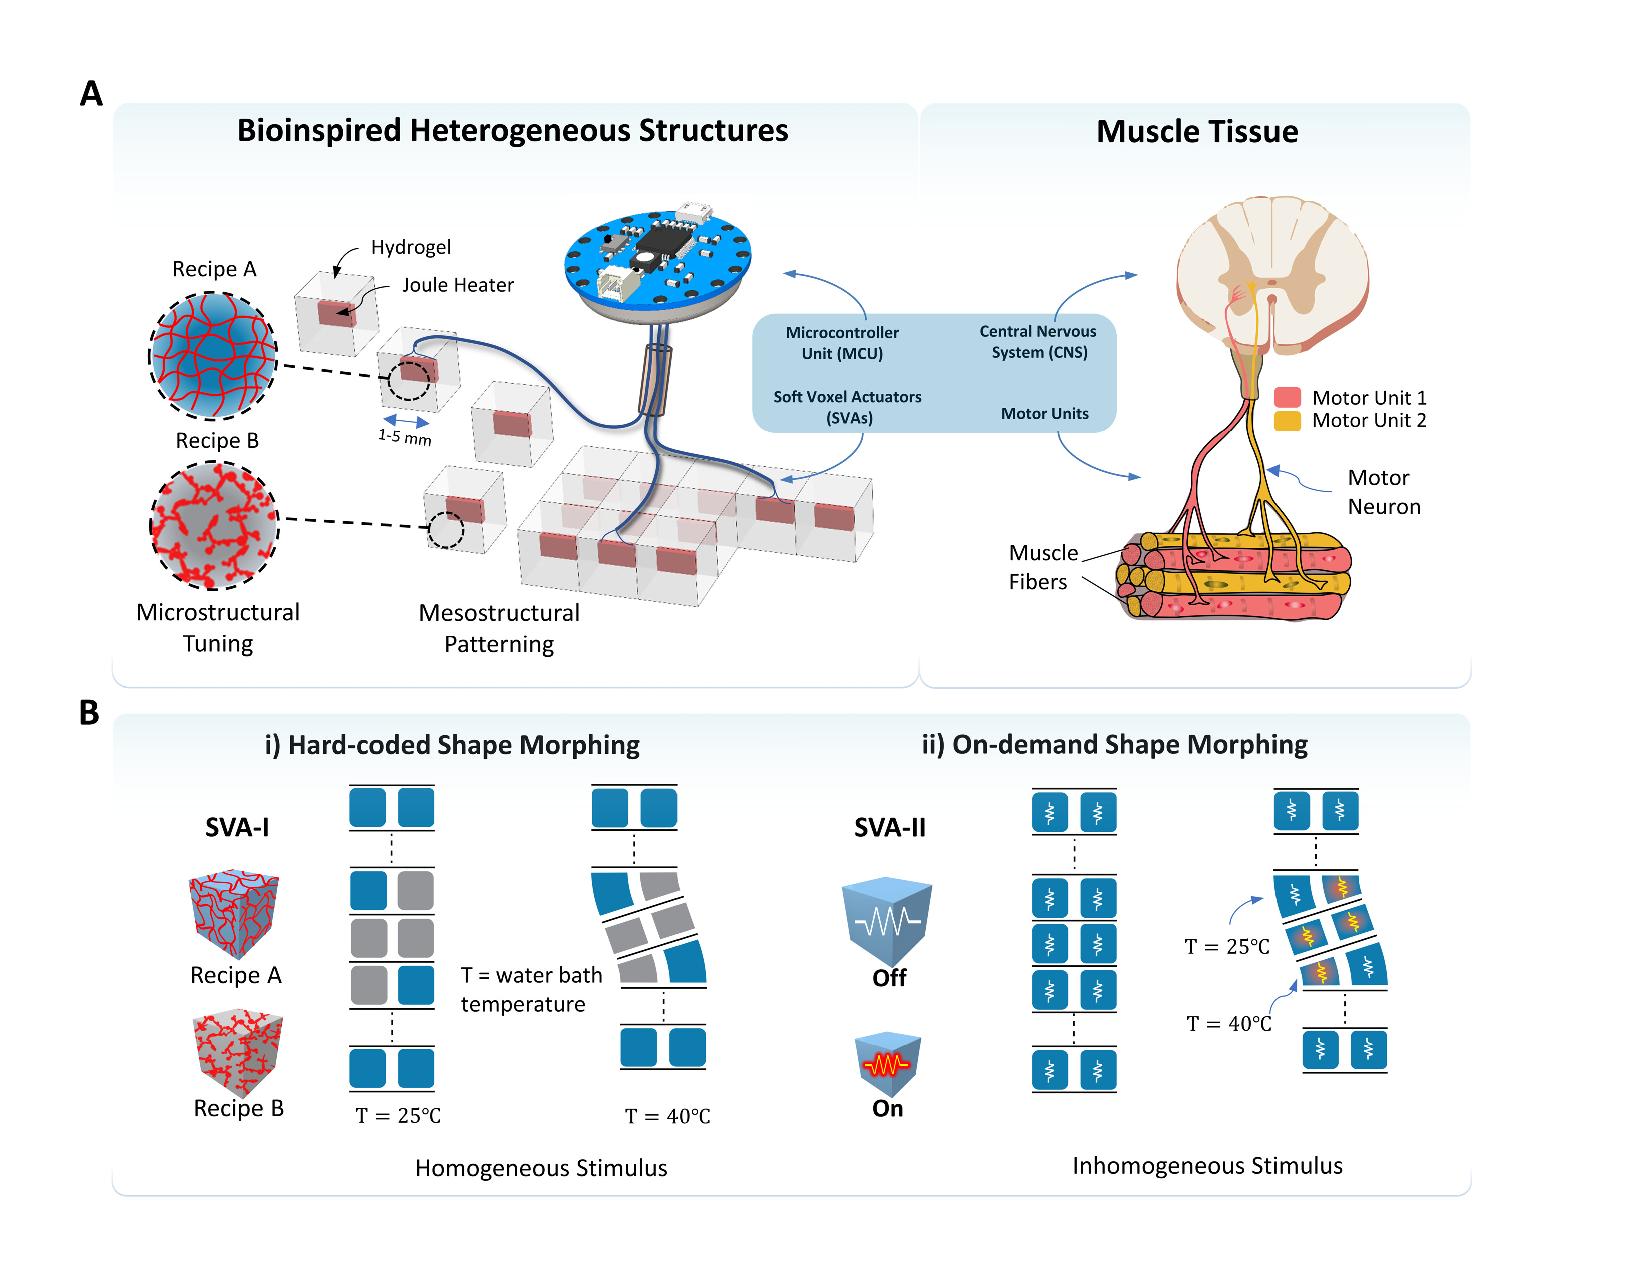
\includegraphics[width=\textwidth]{fig1.pdf}
\caption[Illustration of bioinspired heterogeneous hydrogel structures]{Illustration of bioinspired heterogeneous hydrogel structures composed of tunable and addressable voxels. \textbf{A)} Soft Voxel Actuators (SVAs) are electrically addressable building blocks whose deformations can be controlled by a microcontroller unit (MCU). SVAs are analogous to motor units, consisting of a motor neuron and associated muscle fibers, which deform in response to electrical impulses from the CNS. The microstructure of the hydrogels used to make SVAs can be altered, resulting in tunable material properties. \textbf{B)} i) SVAs without embedded Joule heaters (SVA-I) are used to create structures with hard-coded shape morphing that respond to a homogeneous temperature field acting globally on the entire structure through the surrounding water bath. ii) SVAs with embedded heaters (SVA-II) are used to create structures with on-demand shape morphing by forming an inhomogeneous temperature field throughout the structure.}
\label{fig:1}
\end{figure}

% achieved through altering the microstructure of the hydrogels,
% \note{Tuning the properties is made possible by a hydrogel recipe that supports generating materials with vastly different material properties with only slight differences in the fabrication steps.}
% \xh{I re-structured this paragraph by introducing the needs for a tunable synthesis method, following by a brief overview of current methods, before proposing our method.}
The ability to select from a broad range of material properties for SVA fabrication can expand the design space of resulting heterogeneous structures. Therefore, a synthesis method that can tune the ratio and rate of hydrogel volume change is required. 
% to achieve \sout{hydrogels with} a broad spectrum of swelling properties for creating modular SVA assemblies with efficient motion and dexterity.} 
A variety of physical and chemical methods have been explored to alter the swelling properties of hydrogels \cite{Zhang2008,Imran2010}. 
These methods are limited by factors such as the narrow range of achievable swelling properties \cite{Kim2016,Gan2001}, large trade-offs in mechanical properties \cite{Li2018,Depa2012}, long processing times \cite{Zhou2018b, Ma2014}, and a need for careful control of synthesis conditions such as temperature \cite{Otsuka2012} and precursor additives \cite{Bodenberger2016}.\\ 
%\ya{regarding large trade-offs in mechanical property, our technique does not compromise mechanical property at all, in fact they are enhanced. You can reference our Young's modulus measurements to support this}
% \xh{True? This incapability of tuning is conflict with the previous sentence. Those methods indeed CAN tune the response rate and ratio. Did you mean their tuning range is small? \rk{yes, I meant they can for example make the response fast but they dont discuss that the speed can be set at any desired value over a range}} 
% In addition, these methods are usually time consuming and require careful control of synthesis conditions, which increases the processing time and complexity of the entire fabrication. For example, some synthesis \xh{Too vague. Add a few adj words to describe it and be a bit more specific about what synthesis strategy it is here, rather than talking about the curing time only.} involved 2-hour degassing and 1.5-hour photopolymerization.\citesuperscript{Zhou2018b} Some polymerization takes 24 h to be completed.\citesuperscript{Ma2014} 
% \rk{maybe here I can talk about the requirements of a recipe in order to be a good candidate  for making SVAs such as: mass production (long processing time prevents mass production), compatible with 3D printing methods (should be photopolymerizable,} \xh{OK. The above two examples only talk about the long fabrication time but did not provide information about why. People would wonder what's unique in our method make the curing shorter. Please let me know or use a few adj words before "synthesis" to indicate why, as I commented above. For example, tuning monomer concentration, ratio, or oxygen-free condition...Please do tell.}
% Among these methods, the mixed solvent method appears promising because of the simplicity, fewer processing steps, and inexpensive equipment.\citesuperscript{Wang2017e,Lee2000,Moreno2017} \xh{It seems there are other mixed solvent methods before. How did they work briefly?  Since I restructured this paragraph, this sentence needs to be rephrased.} 

%\xh{add the important benefit of this synthesis method: being able to create interconnected open pore microstructure, which was not reported previously. Such a structure, importantly, significantly enhanced the diffusion of water in and out of the hydrogel matrix and thus led to rapid actuation.} The materials and synthesis technique are described in details in the \note{Supporting Information}.
We take advantage of PNIPAAm's cononsolvency, a property of reduced solvation in a mixture of two solvents due to a delicate balance between polymer-solvent and solvent-solvent interactions \cite{Pica2016}. Employing a water and dimethyl sulfoxide (DMSO) mixed solvent in the PNIPAAm hydrogel precursor solution, followed by rapid photopolymerization to induce interconnected open pores, significantly enhanced the rate of water transport into and out of the hydrogel matrix and thus the actuation speed. The microstructure of the gel is altered by changing the water volume fraction (\(\varphi_{w}\)) in the mixed water/DMSO solvent. The SVA swelling rate and displacement, which are directly related to its hydrogel microstructure, are therefore tuned by merely  adjusting \(\varphi_{w}\). Polymerization solvent composition is known to affect the swelling properties of the synthesized PNIPAAm hydrogels \citesuperscript{Wang2017e,Lee2000, Zhang2002a,Feng2011,Tokuyama2008}. 
%Rapid actuation using hydrogels requires ultrafast swelling speeds; 
The combination of the mixed solvent method with a fast 15\,s photopolymerization step is critical for inducing and fixing local aggregations of polymer chains in place,
% \rk{aggregation of polymer chains(what does it mean)}
resulting in PNIPAAm hydrogels with open pore structures (\firstsubfigref{fig:2}{A(i)}). Such open pore structures exhibit significantly enhanced rates of thermoresponsive volume change in both heating and cooling phases, compared to conventional hours-long mixed solvent thermopolymerization methods (control experiment), in which the precursors are constantly diffusing towards a homogeneous molecular equilibrium throughout the duration of the reaction, leading to a less interconnected pore structure with thicker pore walls (\subfigref{fig:2}{A(ii)}).
In order to ensure a valid comparison, the recipe for a representative thermopolymerized control hydrogel was carefully tuned using the initiator concentration while leaving all other components of the precursor solution unchanged, choosing a reaction time such that the conversion and water content match those of the photopolymerized hydrogel (Supporting Information and Table S2). It is readily observed that with equivalent water content, reaction conversion, and reaction solvent composition, the thermopolymerized hydrogel deswells as fast as the photopolymerized hydrogel \subfigref{fig:2}{B(i)} and the two reach nearly identical shrunken volumes (Figure S8, Supporting Information). However the reswelling speed of the thermopolymerized control sample is $\sim$25 times slower than the photopolymerized sample, which can be attributed to the lower observable tortuosity present in the photopolymerized sample \subfigref{fig:2}{B(ii)}. The Young's Modulus of the thermopolymerized hydrogel is $\sim$10 times higher than that of the photopolymerized one (Figure S9, Supporting Information). \\
%\rk{with have combined some of the favorable features of these methods, focusing on reducing the number of ingredients and shortening the fabrication time in order to make the production of SVAs feasible in labs with less material processing capabilities.}

% UV polymerization has been used to polymerize a hydrogel voxel with dimensions of $4\times4\times4\,mm$ in less than $10\,s$. 

% Therefore, using our proposed mixed solvent method simplifies the entire fabrication of SVAs and assembly of heterogeneous hydrogel structures.
% The mixed solvent method appears promising because of fewer processing steps and inexpensive equipment\citesuperscript{Wang2017e,Lee2000,Moreno2017} which can greatly simplify the fabrication of SVAs. By merely varying the water:DMSO volume ratio denoted by \(\varphi_{w}\), we have been able to tune the swelling properties of poly(N-isopropylacrylamide) (PNIPAAm) hydrogels over a wide range. The materials and synthesis technique are described in details in the \note{Supporting Information}. 
% Using this method, the swelling rate and displacement of SVAs can be tuned by merely adjusting the water volume fraction \(\varphi_{w}\) in a mixed water/DMSO solvent.
% In comparison to the polymerization time in previously reported mixed solvent methods which in some cases approaches 24 h,\citesuperscript{Zhang2002a,Feng2011,Tokuyama2008} \xh{Ref 42 does not have journal name.} our proposed method which uses UV polymerization can be used to polymerize hydrogels in less than 10 s.\xh{Aren't there previous reports that use photo-polymerization with mixed solvent? In another word, are we the first one reporting mixed solvent photopolymerization to prepare hydrogels? } Therefore, using our proposed mixed solvent method simplifies the entire fabrication of SVAs and assembly of heterogeneous hydrogel structures. 
% \xh{I still strongly believe our method is not simpler than others just because of photopolymerization, since nearly all the synthetic hydrogels are photo/thermally-polymerized. Our advantage of this synthesis method is not in the 'simplicity; it is on the effective and continuous tuning of response rate and ratio to provide the choices for SVAs. If we submit to material-topic journals, reviewers likely will question this.}

% defined as:
% $$\varphi_{w} = \frac{V_{w}}{V_{w} + V_{DMSO}}$$
% \note{can't use \textbackslash text\{DMSO\}}  
% The successful realization of such heterogeneous structures lies in our facile hydrogel synthesis method which enables tuning its swelling properties by varying the amount of water in a water/DMSO mixed solvent\note{put action in the front}. 

% \rk{This limitation has prevented the widespread use of many hydrogels with highly desirable properties by robotic researchers.}\note{\citesuperscript{}} 


% \note{Insert into previous paragraph}We have used a water/DMSO mixed solvent and a UV polymerization to synthesize poly(N-isopropylacrylamide) (PNIPAAm) hydrogels. The details of the synthesis technique are described in the supporting information \note{S!}. Using this method, the swelling rate and swelling ratio of SVAs can be tuned by merely adjusting the water volume fraction \(\varphi_{w}\) in a mixed  water/DMSO solvent defined as:

% $$\varphi_{w} = \frac{V_{w}}{V_{w} + V_{DMSO}}$$
% \note{can't use \textbackslash text\{DMSO\}}
% Water volume fraction \(\varphi_{w}\) in a mixed water/DMSO solvent determines the microstructure of the gel. Since the swelling properties are affected by the microstructuer, the swelling rate and displacement of SVAs can be tuned by merely adjusting the 
The effect of varying \(\varphi_{w}\) on the hydrogel microstructure has been investigated by scanning electron microscopy (SEM), as shown in \subfigref{fig:2}{C}. Six hydrogels consisting of various \(\varphi_{w}\) were synthesized; they are each represented by a character code ranging from HG00 (representing a hydrogel with \(\varphi_{w}\) = 0.0) to HG05 (representing a hydrogel with \(\varphi_{w}\) = 0.5). Details of the SEM imaging procedure are described in the Supporting Information. Distinct changes in the microstructure can be observed as a function of \(\varphi_{w}\), which impacts a variety of other material properties. When \(\varphi_{w}\) is increased from 0.0 to 0.2, pore size decreases and the pore wall surface begins to change from smooth to rough. We define \(\varphi_{w}\) = 0.2 as a critical water volume fraction, at which the microstructure of the gel starts to change from a closed-pore to an open-pore structure. SEM images for other values of \(\varphi_{w}\) are presented in Figure S4 in the Supporting Information.
\begin{figure}[t]
\centering
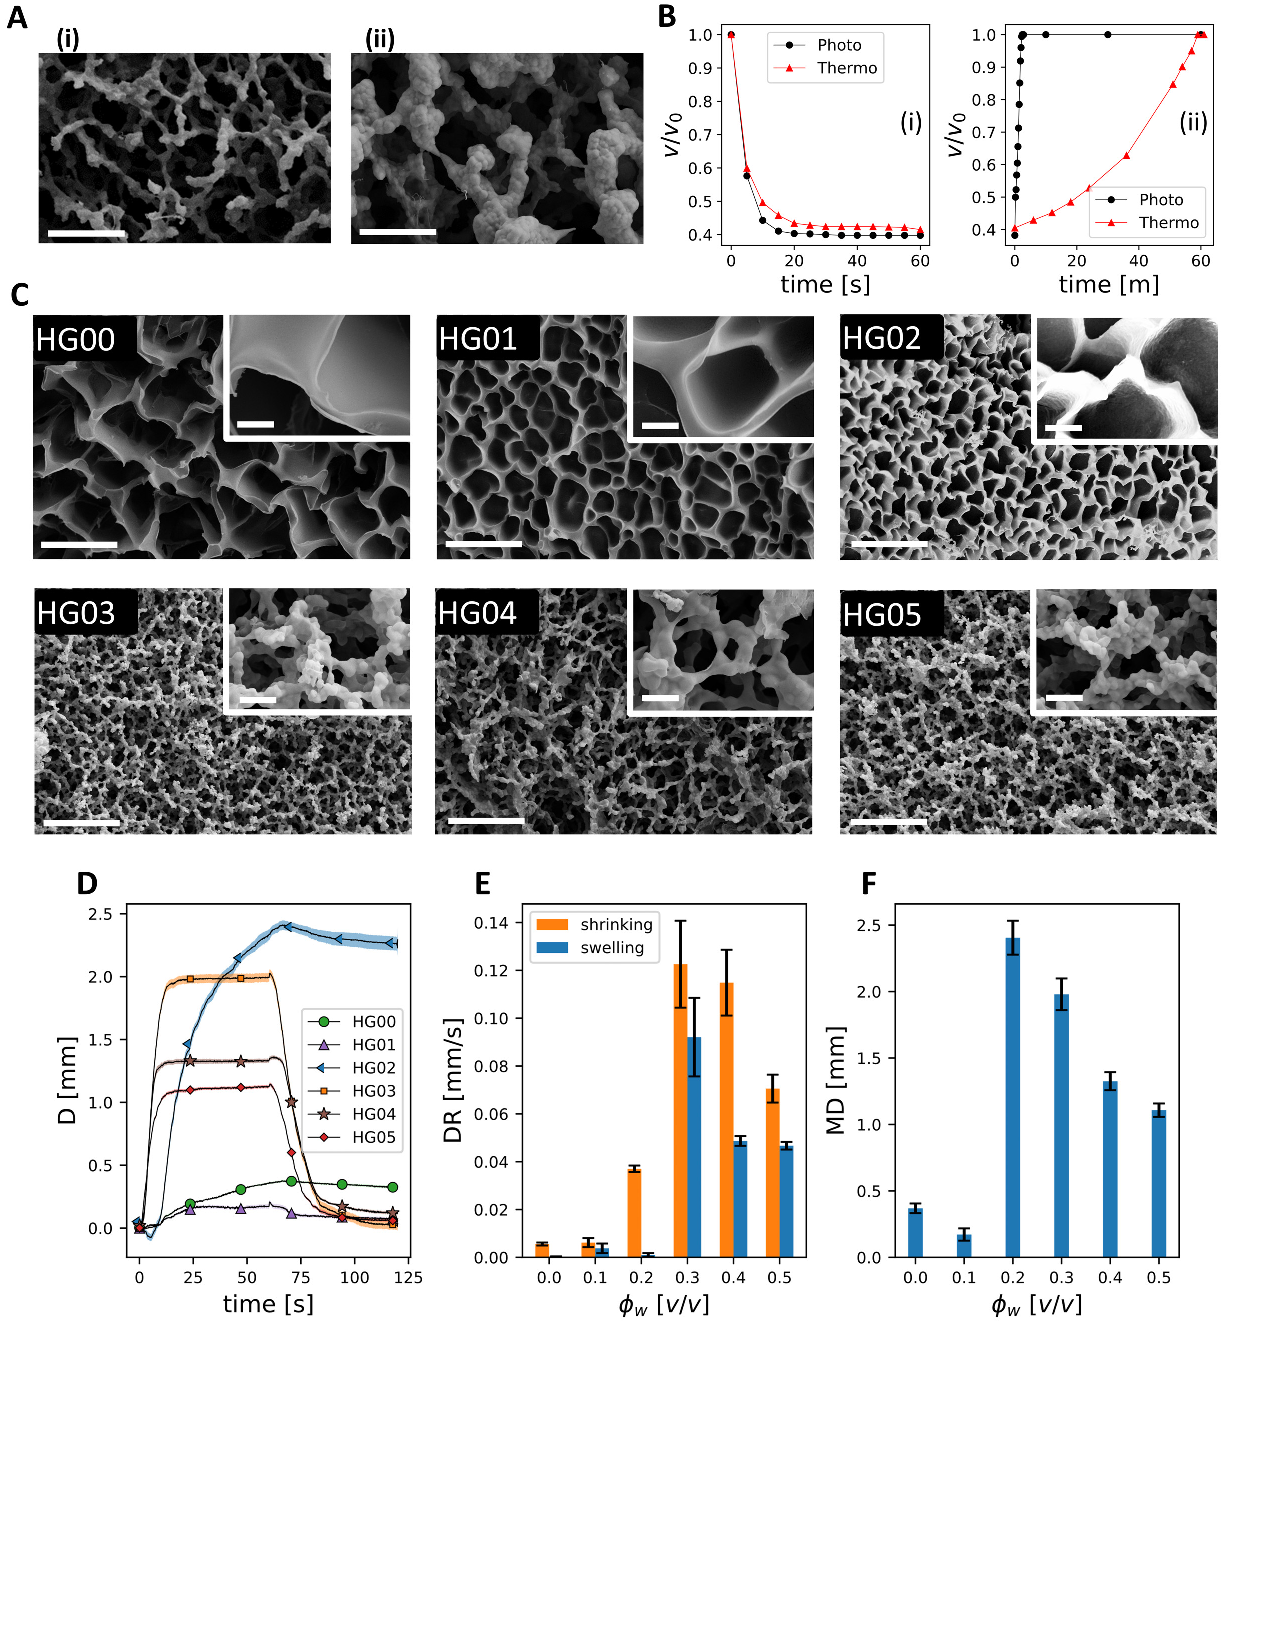
\includegraphics[width=\textwidth]{fig2.pdf}
\caption[Tunable material properties using mixed solvent photopolymerization]{Tunable material properties using mixed solvent photopolymerization.
% achieved by varying water volume fraction ($\varphi_w$) in the prepolymer mixture. 
\textbf{A)} SEM micrographs of photopolymerized (i) and thermopolymerized (ii) hydrogels synthesized in water volume fraction \(\varphi_{w}\)\,=\,0.27 (scale bar = $5\,\mu m$). \textbf{B)} Deswelling (i) and swelling (ii) rates of photopolymerized and thermopolymerized hydrogels synthesized in water volume fraction \(\varphi_{w}\)\,=\,0.27. \textbf{C)} SEM images showing the effect of $\varphi_w$ on pore structure of the photopolymerized PNIPAAm hydrogel (scale bars $10\,\mu m$ and $1\,\mu m$ for low and high magnification, respectively). \textbf{D)} Displacement (D) over time generated by SVA-II units with different values of \(\varphi_{w}\)  under a $1\,gf$ load, as measured by the setup described in the Supporting Information. \textbf{E,F)} Displacement rate (DR) and maximum displacement (MD) of SVA-II units as a function of $\varphi_w$,(extracted from B as described in the Supporting Information).}
% e) Compressive blocked force of a SVA-II f) Maximum compressive force as a function of $\varphi_w$ (extracted from e). 
% g) Young's modulus (E) as a function of SR. the data collection setup is described in methods.\note{change SR to $\varphi_w$}}
\label{fig:2}
\end{figure}
% \rk{this section should be rewritten to account for the fact that we have characterized actuators and not the material}
The changes in hydrogel microstructure play a role in the dynamic response of SVAs. The linear displacement generated by a SVA unit
% defined as the volume of the fully swollen SVA to that of dry gel -- 
is measured using a vision-based test setup as described and shown in the Supporting Information and Figure S3. \subfigref{fig:2}{D} plots the time evolution of the displacement ($D$) of SVA units with different values of $\varphi_w$ 
%as a function of time -- 
as each SVA's embedded heater is turned on for 60\,s 
% \rk{should a space be inserted between the s 60?} \xh{typically yes, between the number and unit} 
and then turned off for 60\,s. The displacement over time of the hydrogel made with \(\varphi_{w}\) = 0.0 is included as the basis for comparison across all tests. The negative displacement observed is because the SVAs initially expand instead of contract as the heater is turned on which might be due to water slightly expanding and vaporizing. Two performance criteria for the SVA units, deformation rate ($DR$) and maximum displacement ($MD$), are extracted from the data in \subfigref{fig:2}{D} and are shown in \subfigref{fig:2}{E,F} respectively. During both heating and cooling, $DR$ is small for \(\varphi_{w} < 0.2\). At \(\varphi_{w} = 0.2\), the $DR$ during heating is more than 36 times the $DR$ during cooling. As a result, fast and large deformations are observed during the 60\,s of heating, and almost no deformation is observed during the 60\,s of cooling. 
Highest $DR$ (in both heating and cooling) occurs in gels with $\varphi_w = 0.3$, while $MD$ peaks at $\varphi_w = 0.2$ and decrease thereafter.
% \note{more, or faster? rate or total shrinkage? use quantitative DR, MD etc..} 
% as the heater is turned on. When the heater is turned off, however, the gel does not swell during the 60s duration of the experiment.
In addition to swelling properties, other mechanical properties such as Young's modulus and force produced by the SVAs can also be tuned by adjusting \(\varphi_{w}\) (Figure S5, Supporting Information).\\ 

% We have used the tunable hydrogel recipe and voxel-based assembly as tools to increase the variety and complexity of shape transformations in heterogeneous structures. Due to the wide range of tunable properties enabled by our hydrogel synthesis technique,
A variety of heterogeneous structures can be produced that transform into different configurations, depending on their hard-coded material domains, as shown in \firstfigref{fig:3}. 
% \rk{add description about why we grouped voxels together and cast them together} 
As a first example, a beam with only two material domains is fabricated from HG00 and HG02 hydrogels (\subfigref{fig:3}{A(i)}). 
% We use this structure as a bench mark to compare the performance of structures produced using our mixed solvent method to those presented in materials science literature\note{\citesuperscript{}}. 
At 20\,$^{\circ}$C, the beam is in its equilibrium position. As the temperature increases to 45\,$^{\circ}$C, the HG02 hydrogel shrinks more than HG00 (from \subfigref{fig:2}{C,D}, both $MD$ and $DR$ are higher for HG02), 
% \note{more or faster?} 
which results in a stress mismatch. To balance these stresses, the beam bends into a circular shape. 
% as seen in \subfigref{fig:3}{A}.
We will henceforth refer to this structure as a `gripper'. %for future reference. 
A second example uses HG00 and HG02 hydrogels again, but this time with 
% a voxel-based arrangement, creating shape morphing structures with multiple 
8 material domains, as shown in \subfigref{fig:3}{B(ii-iv)}. The beams in these figures consist of different arrangements of HG00 and HG02 voxels, and as a result exhibit different deformations when subjected to a homogeneous temperature change in the surrounding water from 20\,$^{\circ}$C to 45\,$^{\circ}$C (for details, see Movie S1 in the Supporting Information)\\
% The wide range of tunable properties enables creating heterogeneous structures with complex functions. \rk{add description about why we grouped voxels together and cast them together} As a first step, a bilayer beam -- a commonly used structure demonstrated throughout materials science literature\note{\citesuperscript{}} -- is created with HG00 and HG03, as shown in \firstsubfigref{fig:3}{A}. This beam bends to one side as the temperature increases because the HG03 hydrogel shrinks more \dma{than HG00}\note{more or faster?} according to \subfigref{fig:3}{A}. Further, our proposed voxel-based approach has also been used to create shape morphing structures as shown in \subfigref{fig:3}{B}. Different voxel arrangements using HG00 and HG02 deform when subjected to a homogeneous temperature change in the surrounding water from 20 to 45\textsuperscript{o} C.

Patterning material domains can be used to leverage the shape transformations into unique functions tied to structural heterogeneity.
% A combination of voxels made of HG00, HG02 and HG03 to increase the complexity of generated shapes even further bilayer and voxel-based structures to perform even more complex tasks. 
% At this level, these heterogeneous structures may be considered soft robots, since they can perform functions such as grasping and manipulation. \note{out of place}
To demonstrate this \textit{structure--function} relationship, two different structures, Str-I and Str-II, are made with different combinations of HG00, HG02, and HG03, as shown in \subfigref{fig:3}{B}. These structures represent a combination of the structures in \subfigref{fig:3}{A}(i,ii). 
% and are shown in \subfigref{fig:3}{A,B}.
% Two different structures  -- Str-I and Str-II --  have been constructed which are shown in top and bottom row of \subfigref{fig:3}{c} respectively. 
In response to a global cyclic temperature change from 20\,$^{\circ}$C to 45\,$^{\circ}$C
% \textsuperscript{o}C 
and back to 20\,$^{\circ}$C, these structures are observed to bend towards an object, grasp it (by wrapping around it), and transport it to another location (\subfigref{fig:3}{B} and (Movie S2, Supporting Information). The geometric configuration of material domains in both structures are the same. However, the `gripper' portion of Str-I is a combination of HG00/HG03 domains, whereas in Str-II it is a combination of HG00/HG02 domains. As a result of this minor material difference, the object grasped by Str-I and Str-II moves along different trajectories, as seen in \subfigref{fig:3}{C}, despite an identical set of initial conditions. Due to the high $DR$ of HG03  
% in the gripper part of Str-I 
during the cooling phase (\subfigref{fig:2}{E}), the gripper in Str-I opens and the object is released in the early stages of the cooling phase. 
% (\note{Movie S5, Supporting Information}). 
The gripper in Str-II, on the other hand, does not open at the same time as Str-I and continues to hold the object throughout its cooling phase; this can be attributed to the lower $DR$ of the HG02 layer compared to HG03. To illustrate these differences, the $x$ and $y$ coordinates of the object over time are plotted %depicted 
in \subfigref{fig:3}{D}, and the time when the object is released by each structure is indicated. Achieving inhomogeneous deformations in response to a homogeneous global stimulus using structures with hard-coded deformations as described simplifies the system and eliminates the need for on-board power sources.\\ 

\begin{figure}[t]
\centering
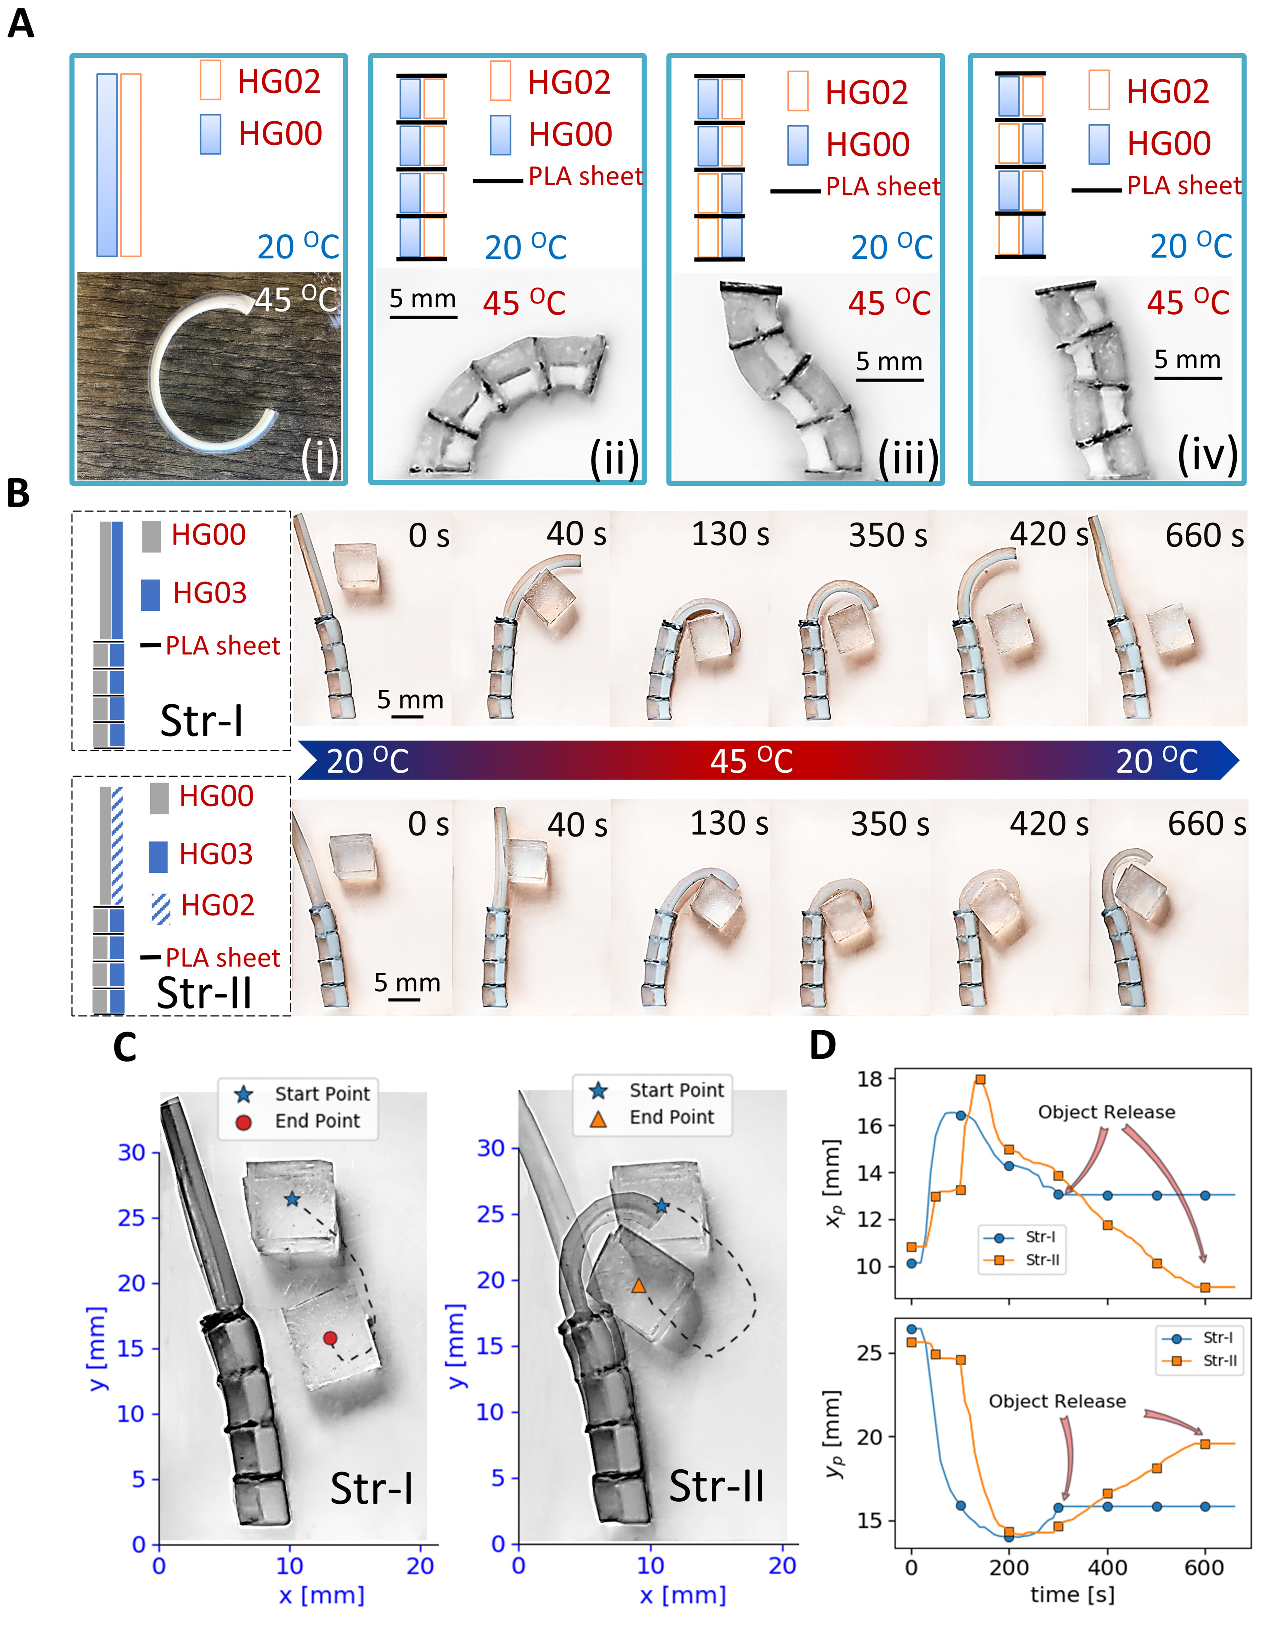
\includegraphics[width=\textwidth]{fig3.pdf}
\caption[Realization of structural inhomogeneity]{Realization of structural inhomogeneity through patterning of hydrogels with different swelling properties. \textbf{A)} (i) A two-material, two-region structure can almost bend into a circle when the surrounding water bath temperature is raised  above the transition temperature of PNIPAAm hydrogel (~32\,$^{\circ}$C) (ii-iv) Increasing the number of material domains in the structure enables it to achieve more diverse shapes. When the surrounding water bath temperature is increased, each structure reconfigures into a different shape, depending on its arrangement of SVA-I units. \textbf{B)} Hybrid structures comprised of substructures with the SVA arrangements in A)(i,ii) are
%Using \spr{\sout{the structures}  the SVA arrangements} introduced in A), hybrid structures are \spr{created that are \sout{made}} 
capable of manipulating objects. The material distribution in two example structures, denoted by Str-I and Str-II, is shown in the schematic on the far left. The snapshots display the configurations of the two structures over time as the global water bath temperature is increased and then decreased.
% the top row denoted by Str-I is made of a bilayer comprising HG00 and HG03 whereas in the bottom row (Str-II) is composed of HG00 and HG02. 
\textbf{C)} Image showing the start position,  end position, and  trajectory of the  object manipulated by Str-I (left) and Str-II (right). \textbf{D)} Time evolution of the $x$ and $y$ coordinates of the manipulated object's center of mass.  Str-I releases the object   a $t=300$ s, while  Str-II releases it at $t= 600$ s, demonstrating the versatility of the voxel-based assembly approach to creating heterogeneous structures with diverse functions.}
\label{fig:3}
\end{figure}

For applications in dynamic, unstructured environments, such as underwater robotic exploration, it is less useful to pre-program complex trajectories into a structure, since global stimulus control is not always feasible. To enable on-demand thermoresponsive shape morphing in these conditions, SVA-II units may be employed, as depicted in \subfigref{fig:1}{B(ii)}. The 40×11×5 mm structure shown in \firstsubfigref{fig:4}{A} was assembled using 16 SVA-II units. These SVAs are made of HG03, which exhibits the highest $DR$ observed across all recipes (\subfigref{fig:2}{E}). The first example of on-demand shape morphing is illustrated in \subfigref{fig:4}{B(i)}, in which the structure morphs into an `S' shape and a `reverse S' shape when particular SVAs are actuated via commands from a microcontroller. %where the same structure morphs into `S' and `reverse S' shapes based on commands from a microcontroller. 
A second example of on-demand shape morphing is illustrated in \subfigref{fig:4}{B(ii)}; it highlights how the curvature of a structure may be varied as a function of the voltage supplied to the SVA-II units.\\

Moving from static to dynamic on-demand shape changes requires time-varying activation of SVAs.
As demonstrated in \subfigref{fig:4}{C}, the choice of SVA actuation pattern can influence the end-effector trajectory of a structure. In this experiment, SVAs 1 thorough 8 are activated according to patterns denoted by P1 and P2.
% in \subfigref{fig:4}{D}. 
Each SVA is activated with maximum voltage (3.7\,V) for 15\,s before the next SVA is activated, as shown in \subfigref{fig:4}{C} 
and Movie S3 in the Supporting Information.\\  


%the assigned tasks are achievable with our technique.
% Therefore this SVA assembly can successfully operate in unstructured environments, in which working conditions may change during operation. The details of this structure in interacting with the environment can be seen in \note{video S}. 
% In each situation, different trajectories should be followed by the tip of the manipulator denoted by point p in the coordinate system O in \subfigref{fig:4}{A}. These trajectories are shown in \subfigref{fig:4}{E}. 
% vary only slightly and the manipulator should be capable of performing precise movements in order to follow such trajectories. 
% \subfigref{fig:4}{A}

%In the previous demonstration, only on and off states (corresponding to an activation voltage of 0 $V$ and 3.7 $V$ respectively\note{on and off or off and on?}) were used to demonstrate complex trajectory generation. 
%While as in 
While complex motion of SVA-II-based structures may be achieved using simple on 
(3.7\,V) and off (0\,V) activation signals, as discussed,
intermediate voltages may also be applied to further enhance the complexity of shape change in soft heterogeneous structures. To demonstrate this, phase-shifted sinusoidal voltages were used as activation signals to generate longitudinal traveling waves in the structure. 
% \spr{\sout{selected} (I thought that only every other pair was activated, but the caption implies that some voltage plots were not shown, so were all SVAs except 4 and 12 activated?)}
A pair of SVAs (comprising a SVA on the left and its adjucent SVA on the right) are activated using the same sinusoidal signal; SVAs 4 and 12 were not activated, to serve as a geometric reference point.
% All pairs of SVAs, except SVAs 4 and 12, 
 The sinusoidal voltages applied to every SVA pair were $\frac{\pi}{8}~rad$ out of phase with the voltages applied to its nearest active SVA pair. As an example, sinusoidal signals for four SVA pairs are shown in  \subfigref{fig:4}{D}. 
%  (The figure shows that there is a phase shift of $\pi/8$ between every {\it other} pair of SVAs. Is it between adjacent pairs of SVAs? Or is the phase shift $\pi/16$ between adjacent pairs?)}
%compared to their adjacent pair. 
%SVA pair  comprising
 A contraction wave was formed as a result of this input signal pattern and traveled along the length of the structure, as illustrated in \subfigref{fig:4}{E}. Movie S4 in the Supporting Information shows in detail how these waves are generated and propagated along the structure. Every point on the structure oscillates in a sinusoidal manner as the wave passes through it. The midpoint of the inactive SVA pair, which is highlighted by a yellow square in \subfigref{fig:4}{E}, is shown as a reference point on the structure. Additionally, by sending the sinusoidal signals to SVAs located on only one side of the structure, for example SVAs 1 through 8, transverse traveling waves were generated in the structure (Movie S4, Supporting Information).
% The sequence of electrical control signals used to operate the structure in performing the two tasks are shown in \subfigref{fig:4}{\note{?}}.
The ability to control the trajectory of the structure's end-effector, as shown in \subfigref{fig:4}{C}, is essential to successful functioning of the device in unstructured environments, in which working conditions may change during operation.
% As an application, We may furthermore show how the sequential activation can be used to create different trajectories followed by the tip of the structures on-demand using resulting in successful operation in unstructured environments, in which working conditions may change during operation. 
%As seen in the upper row of \subfigref{fig:4}{F}, \dma{SVA-II structures may \sout{this structure can}} be \dma{\sout{commanded by the control signal from a microcontroller to follow a specific trajectory necessary to avoid collisions with obstacles placed within its workspace}}\note{update subfig refs}. 
As depicted in \subfigref{fig:4}{F},  time-sequenced switching of selected SVA-II units within the structure makes it possible to accomplish various robotic tasks such as collision avoidance (top row) and object transport (bottom row).
% Based on activation signal of each SVA unit, different trajectories are followed by end effector $p$ in coordinate system O (as denoted in \subfigref{fig:4}{A}) resulting in the end effector passing over an object and then pushing it left. 
The trajectory of the end point $p$ and the angle $\theta$ of the end plate over time ($p$ and $\theta$ are defined in \subfigref{fig:4}{A}) during each of these two tasks %these two motions
is displayed  in \subfigref{fig:4}{G}. The on-demand control of reorientation and translation of the end-effector made it possible to complete these two tasks, %this two-part task possible, 
indicating that highly redundant time-varying deformations in heterogeneous structures are achievable using individually addressable SVA-II units (Movie S5, Supporting Information).
% necessary for successful completion of complex tasks such as this.
\begin{figure}[t]
\centering
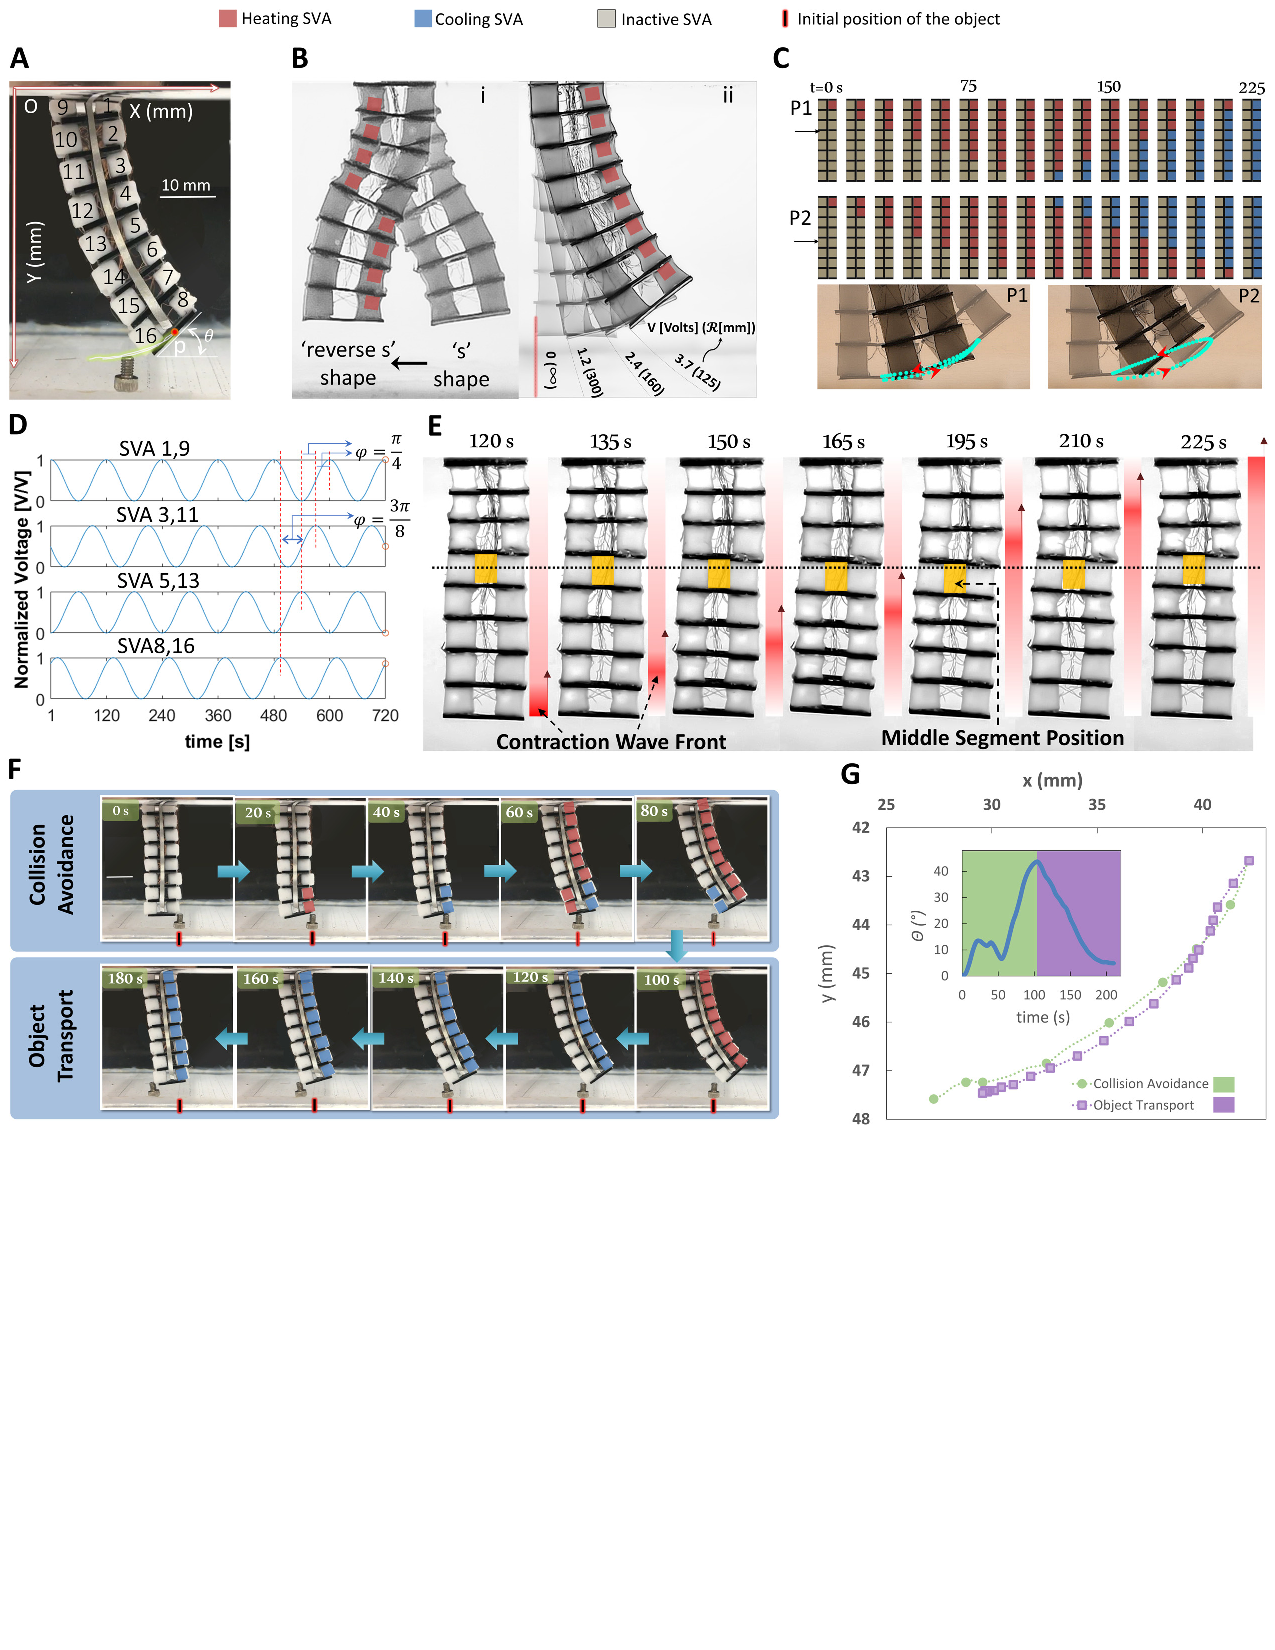
\includegraphics[width=\textwidth]{fig4.pdf}
\caption[A miniature soft robot consisting of 16 addressable SVA-II units]{A miniature heterogeneous structure consisting of 16 addressable SVA-II units. \textbf{A)} SVA numbering scheme and the coordinate system used to measure the position of the point $p$ and the angle $\theta$ of the end plate. \textbf{B)} On-demand shape morphing of the structure. i) The structure morphs from an `S' shape to a `reverse S' shape when particular SVAs are activated. 
%by activating different SVAs. 
ii) The structure's radius of curvature ($\mathcal{R}$) depends on the activation voltage ($V$) applied to SVAs 1-8. \textbf{C)} Dynamic shape changes are implemented by sequentially activating SVAs. In this case, SVAs 1 through 8 are activated according to the patterns labeled P1 and P2. The trajectory followed by the tip of the structure (shown at the bottom) can thus be adjusted on-demand. For details, see Movie S6 in the Supporting Information. \textbf{D)} 
% Taking advantage of the simplicity of creating complex electrical control signals as opposed to other signals such as light, using a microcontrollerThe complex 
Normalized sinusoidal voltages used to create longitudinal traveling waves in the structure. The voltages applied to 8 of the 16 SVAs are shown here. The SVAs are activated in pairs, and the voltage applied to each SVA pair is $\frac{\pi}{8}~rad$ out of phase with respect to the voltage applied to the next active pair. 
% \spr{(or is the phase shift $\pi/8$ between every other pair? see my comment in the main text)}
\textbf{E)} The longitudinal traveling wave as it propagates through the structure. One SVA pair, indicated by the yellow square, is kept inactive in order to serve as a reference point. For details, refer to Movie S7 in the Supporting Information. \textbf{F)} Example usage of heterogeneous structures with on-demand control of deformation. The structure can avoid collisions with objects or transport them, depending on the sequence of voltage commands from the microcontroller unit. \textbf{G)} Trajectory of the point $p$ on the tip of the structure as it first avoids and then transports the object. The inset shows the angle $\theta$ of the end plate as a function of time.}
% In comparison to structures with hard-coded deformations presented in \figref{fig:3}, 
% of the manipulator can follow arbitrary trajectories according to the requirements of the task. The top row is a time-lapse of the manipulator trying to avoid the obstacle. Bottom row is a time-lapse of the manipulator trying to move the object to the left. b) A close-up view of the manipulator with end point p, end plate angle θ and coordinate system used for measuring them. c) The trajectory followed by point p is shown in the middle. Time-based plots of the x and y coordinates of point p and end plate angle θ are shown at the top and bottom respectively.}
\label{fig:4}
\end{figure}

\section{Conclusions}
To summarize, we have developed the following tools to increase the variety and complexity of shape transformations in heterogeneous hydrogel structures: a voxel-based assembly design for patterning material domains, and a unique mixed-solvent photopolymerization hydrogel synthesis method for tuning swelling properties of the voxels. These tools offer a higher number of design parameters, namely, the configuration of the voxels, the material properties of each voxel, and the activation voltage of each voxel (in the case of SVA-II). This rich set of design parameters can be specified to build structures that meet the requirements of a variety of tasks. The resulting heterogeneous structures can generate complex time-varying trajectories and traveling waves, enabling them to interact with unstructured environments in ways that could not be realized in bulk hydrogels or that would require sophisticated integration and manufacturing.\\

The simplicity of these tools advances the utility of hydrogel structures in robotics applications in a meaningful way because they can be used in robotics research laboratories that lack sophisticated material processing facilities.
% The impact of our work lies in bridging the gap between material science and soft robotic fields. Currently, there are several hydrogels with desirable properties such as fast response and high strength which due to their sophisticated preparation process and lack of proper manufacturing techniques, are hard to be used by soft roboticists. Using methods presented in this paper, these hydrogels can be made into voxel building blocks by material processing labs and supplied to robotic researchers who can put them in different soft robotic applications. 
% Due to the wide range of tunable properties enabled by our hydrogel synthesis technique, 
% A variety of heterogeneous structures can be produced that transform into a unique shape, depending on their hard-coded material domains. 
% We have created structures that create more complex configurations and trajectories.  this is facilitated by the approach of using multiple materials and locally controlling the deformation.  
% this backed-up by a facile recipe, together enabled the creation of heterogeneous hydrogel structures that show more complex pre-programmed as well as on-demand deformations.
% These deformations are more complex because we have more control over material distribution by thoughtful placement of different voxels into an assembly, thereby creating heterogeneity in the structure (SVA-I). Addressable voxels that take advantage of an embedded Joule heater enable on-demand deformations, removing the need for creating multiple hard-coded structures to perform different tasks (SVA-II). One structure can perform different tasks. Our recipe also allows facile mass production of voxels as well as tuning the material properties of each voxel.
%Limited supply of our developed soft voxel actuators for research purposes are also available upon request at www\ldots{}.
While this paper focuses specifically on PNIPAAm hydrogel voxels, soft and rigid voxels made of other types of responsive or non-responsive materials can also be incorporated into heterogeneous assemblies. Closed-loop control of the deformation of the structures presented in this paper could be achieved by integrating strain- and force-sensitive voxels, made of similar functional hydrogels, that serve as sensors. In addition, multi-objective optimization across material properties and voxel configurations can be used to design structures with higher force production capacity and %higher 
energy efficiency. Currently, integrating multiple active degrees of freedom (DOFs) in miniaturized soft robots is challenging due to space limitations. Each SVA can be considered as an active DOF and we have demonstrated that the integration of a high number of SVAs in a small footprint, such as the 16-voxel structure presented in this paper, is possible. To address the challenges of fabricating large-scale 
assemblies consisting of hundreds of voxels, % is still challenging and
automated methods must be developed for scalable manufacturing and assembly of voxels.